\graphicspath{{chapters/MethylationImages/}}


\chapter{Epigenetic profiling of cell-free DNA}
Gian Marco Franceschini -  \textit{gian.franceschini@unitn.it}


\section{Introduction}

All the cells of the human organism present the same genetic information but
they give rise to different types of tissues and cells. This happens mostly
thanks to epigenetics. The main epigenetic modifications are:
\begin{itemize}
    \item \textbf{DNA methylation}: in humans they are mainly found on CpG
    islands (genomic regions with high CG content)
    \item \textbf{Histone post translational modifications} (PTMs)
    \item The \textbf{chromatine architecture}
    \item ...and many others
\end{itemize}


All levels of epigenetic controls are often dysregulated in cancer: these
variations usually go in favor of cancer cells survival. For this reason,
epigenetic reprogramming has recently been added to the hallmarks of cancer.

The epigenetic landscape is very different from the genetic one. DNA mutations
are directional: they cannot be reverted so they accumulate with subsequent
cells generations. The epigenome is plastic, so it can be reverted (possibly
through therapy but this can happen physiologically). Moreover, the human
epigenome is tissue/cell specific while the genome is unique.

\section{DNA methylation}

DNA methylation is the addition of methyl-groups to cytosines in CpG islands. It
is regulated by enzymes that are responsible for regulating the cell-specific
transcriptional state. These enzymes can be:
\begin{itemize}
    \item Cis-factors: local control
    \item Trans-factors: genome-wise control
\end{itemize}

CpG islands are spread through the genome and when they are in a promoter they
regulate gene expression through transcriptional silencing of the corresponding
gene if they are methylated. The mechanisms are multiple and still not
completely clear: DNA methylation could for example impair the binding of
transcription factors or recruite repressing proteins. This methylation
landscape is highly regulated and tissue-specific.

In cancer tissue, hypomethylated and hypermethylated regions are often observed,
leading to an abnormal regulation of gene expression. In addition to that,
hypermethylation of pericentrometric heterochromatin in cancer can lead to
mitotic recombination and thus genomic instability \ref{fig:cancer}.

\begin{figure}[H]
\centering
    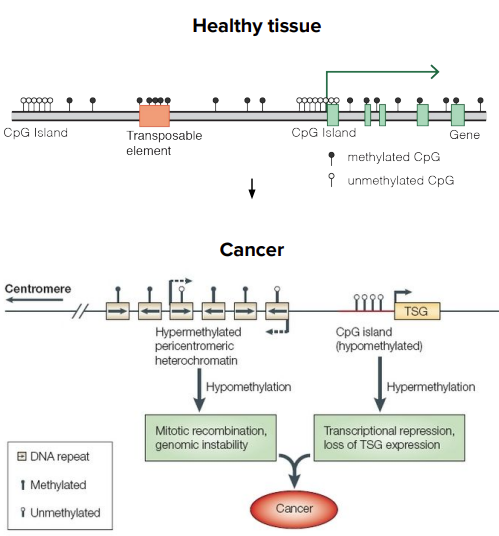
\includegraphics[width=0.5\linewidth]{cancerMet.png}
    \caption{Methylation patterns altered in cancer}
    \label{fig:cancer}
\end{figure}

This landscape of regulation is very complex: DNA methylation can regulate gene
expression but it is not the only regulating factor, some histone modifications
also contribute for example.

DNA methylations are not inherited across generations, so there is no
accumulation of methylation variants, as it happens with regular DNA mutations.
Each individual is born with a brand new methylation landscape that is then
disrupted during life (not only due to cancer or disease). Interestingly, i
could be possible to exploit variations in the DNA methylome to measure age by
computing how many cell divisions led to that specific methylation state.

\section{How is DNA methylation measured?}

The fist step is the \textbf{bisulfite conversion}: thanks to bisulfate ions,
unmethylated Cs are converted into Us. With some particular alignment algorithms
that are aware of these modifications one can detect the errors and thus
methylations. Both array-based and shotgun-sequencing-based assays are used to
this aim. The result of such an assay is a series of \textbf{beta values}: the
fraction of reads corresponding to one genome site that is methylated.

\begin{figure}[H]
\centering
    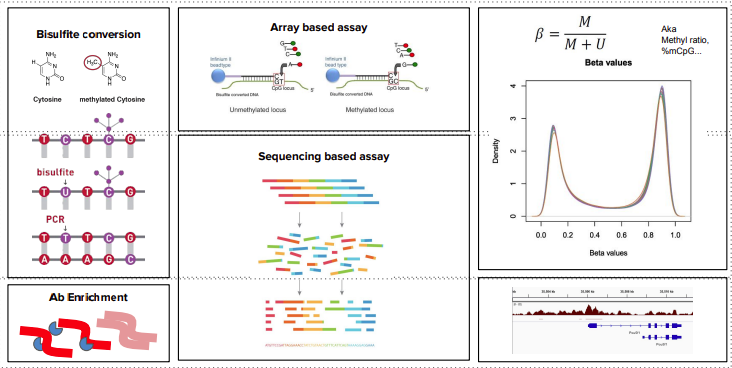
\includegraphics[width=0.8\linewidth]{methods.png}
    \caption{Main methods for DNA methylation measurement}
    \label{fig:met}
\end{figure}

Immunoprecipitation-based methods are also available, but the most frequently
used methods are based on whole genome profiling.\\

It is useful to analyze the sequencing result at the \textbf{single-read level}:
different methylation configurations can lead to the same global methylation
level but have different biological interpretations. For example one methylation
level of 0.5 can be the result of one completely methylated allele with the
other one unmethylated or two half-methylated alleles. This kind of information
is important in order to determine, for example, if the sample contains
different types of cells or if it there is some disrupting pathological
situation.


\section{Tissue-specific vs disease-specific DNA markers}

\begin{itemize}
    \item \textbf{Aspecific} → most of the genome
    \item \textbf{Tissue-specific} → methylations that regulate gene expression
    to activate the tissue-specific functions of cells
    \item \textbf{Disease-specific} → CpG hypermethylation, genome-wide
    hypomethylation and other modifications usually correlated with cancer
    \item \textbf{Tissue+cancer-specific} → methylation patterns specific of
    cancer in a certain tissue. These markers allow to discriminate between
    different tumor types.
\end{itemize}

\section{DNA methylation based liquid biopsy}

When a cancer cell dies, its DNA is released in circulation and it is
potentially possible to get it with a liquid biopsy. The goal is to analyze
methylations of cfDNA to retrieve information about the state of the patient,
and possibly detect early-stage tumors.

For this purpose, when compared to genomic DNA, the analysis of the methylation
landscape has some positive and some negative aspects. For genomic DNA, the
percentage of actually informative signal on the whole information that is
obtained can be small and difficult to observe, on the other hand, for DNA
methylations it is difficult to discriminate between what is aberrant and what
is not because the modifications are tissue-specific and it is difficult to
obtain clear background references to make a comparison.

\begin{figure}[H]
\centering
    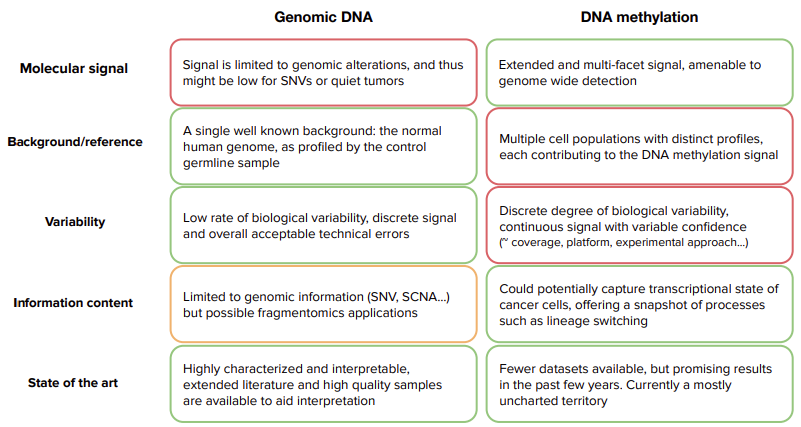
\includegraphics[width=\linewidth]{comp.png}
    \caption{\label{fig:comp}Comparison of genomics vs methylation for cancer
    detection}
\end{figure}

\subsection{Workflow}

First, the data is sequenced from solid and liquid samples: the methylation
profiles from solid samples are needed as reference. The reference profiles for
liquid biopsies analysis are derived from white blood cells and from the cancer
type of interest. White blood cells are the background reference for cfDNA,
since the most frequent genomic material in circulation originates from this
type of cells. If a methylation pattern different from the one of blood cells is
found in cfDNA it means that cells of some other tissue are dying and their
material is going into circulation and it is not a positive signal. With these
pattern as reference, the goal is to discover biomarkers and perform feature
selection. Subsequently, a model is fitted and optimized to perform predictions
on new data. The last step is performance evaluation.

\begin{figure}[H]
\centering
    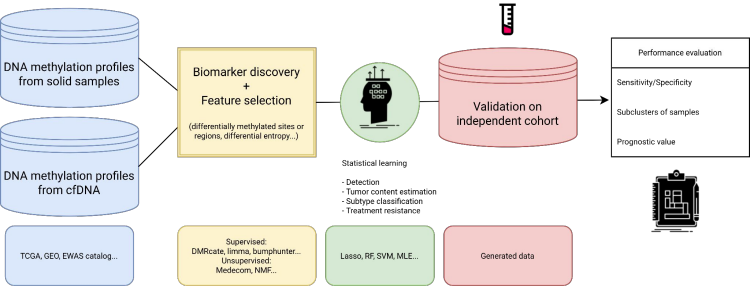
\includegraphics[width=0.8\linewidth]{workflow.png}
    \caption{\label{fig:wo}Common analysis workflow}
\end{figure}

\subsection{CCGA study}

The Circulating Cell-free Genome Atlas (CCGA) is a study conducted by Grail
designed to characterize the landscape of genomic cancer signals in the blood of
people with and without cancer. The study enrolled approximately 15,000
participants. Their goal is early and simple detection of cancer from analysis
of methylations on cell-free DNA.

They performed whole genome methylation profiles after choosing between three
different independent methods (the other two were targeted sequencing and whole
genome sequencing for CNVs but they decided to further develop the methylation
path). In the second phase they developed an assay for a targeted methylation
study: the best features to discriminate between the two classes (cancer vs
non-cancer) were selected in order to sequence the areas with these
modifications without whole genome analysis. A model for this classification was
developed, trained and validated. The last step is a large-scale clinical
validation with a 5 years follow-up that is still in progress.

The results are great but not for all cancer types: sensitivity is better for
cancers of highly-vasculated tissues and metastatic tumors, while some types of
cancer produce a lot of false negative results. Moreover, detection is obviously
better when cancer progresses but the goal is early detection.


\subsection{Deconvolution approaches}

Deconvolution of cell-free DNA is another task to be performed on DNA
methylation other than classification. The goal is to explain the observed
signal with a combination of pure signals: discover the main contribution that
led to a specific methylation landscape, one example is tumor profiling.

From liquid biopsies, it is possible to detect which are the main contributors
to the cfDNA. These results can be compared with the ones obtained from cancer
patients to determine which are the contributors to the difference in cfDNA that
is observed and to infer data for tumor disgnosis or treatment resistance
detection.

In order to perform deconvolution, \textbf{high-quality reference atlases} are
needed: one was built with the contribution of
\href{https://www.biorxiv.org/content/10.1101/2022.01.24.477547v1}{Grail}. They
sorted healthy donors cells with FACS and profiled them. Cell type specific
metylation profiles were built, so it is possible to use this atlas to select
biomarkers, like a reference genome. They generated specific methylation
patterns for 39 human cell types from 207 methylomes.

\section{Targeted panel approaches for tumor content estimation}
\textit{Demichelis'group study}\\

Their interest is detection of treatment resistance in prostate cancer. The goal
is to know when the tumor becomes resistant, in order to be able to change or
calibrate the therapy. A sequencing panel was developed to detect the amount of
cancer-derived DNA in circulation, and interestingly only 50 regions are
sufficient to get a satisfying estimation. A model is built to know how much
ctDNA is expected after treatment and it is possible to get a score that
estimates the level of resistance.
